\subsection{Transform\'ee de Hough}

\subsubsection{Introduction}
La transform\'ee (ou transformation) de Hough est une technique de reconnaissance de formes invent\'ee en 1962 par Paul Hough. \\
L'application la plus simple permet de d\'etecter les lignes/droites pr\'esentes dans une image mais des modifications peuvent \^etre apport\'ees \`a cette technique pour d\'etecter d'autres formes g\'eom\'etriques (cercles, ellipses...) : c'est la transform\'ee g\'en\'eralis\'ee de Hough d\'evelopp\'ee par Richard Duda et Peter Hart en 1972. \\
Cette technique est devenue un outil standard dans le domaine de la vision artificielle.

\subsubsection{Principe}
Le probl\`eme pos\'e est celui de la recherche et de la d\'etection de lignes qui seraient \'eventuellement pr\'esentes dans une image \`a analyser. Le principe de la transform\'ee de Hough est qu'il existe un nombre infini de lignes qui passent par un point, dont la seule diff\'erence est la pente a, l'orientation, l'angle... Le but de la transform\'ee est de d\'eterminer lesquelles de ces lignes sont les plus pr\'esentes dans l'image analys\'ee.
\begin{center}
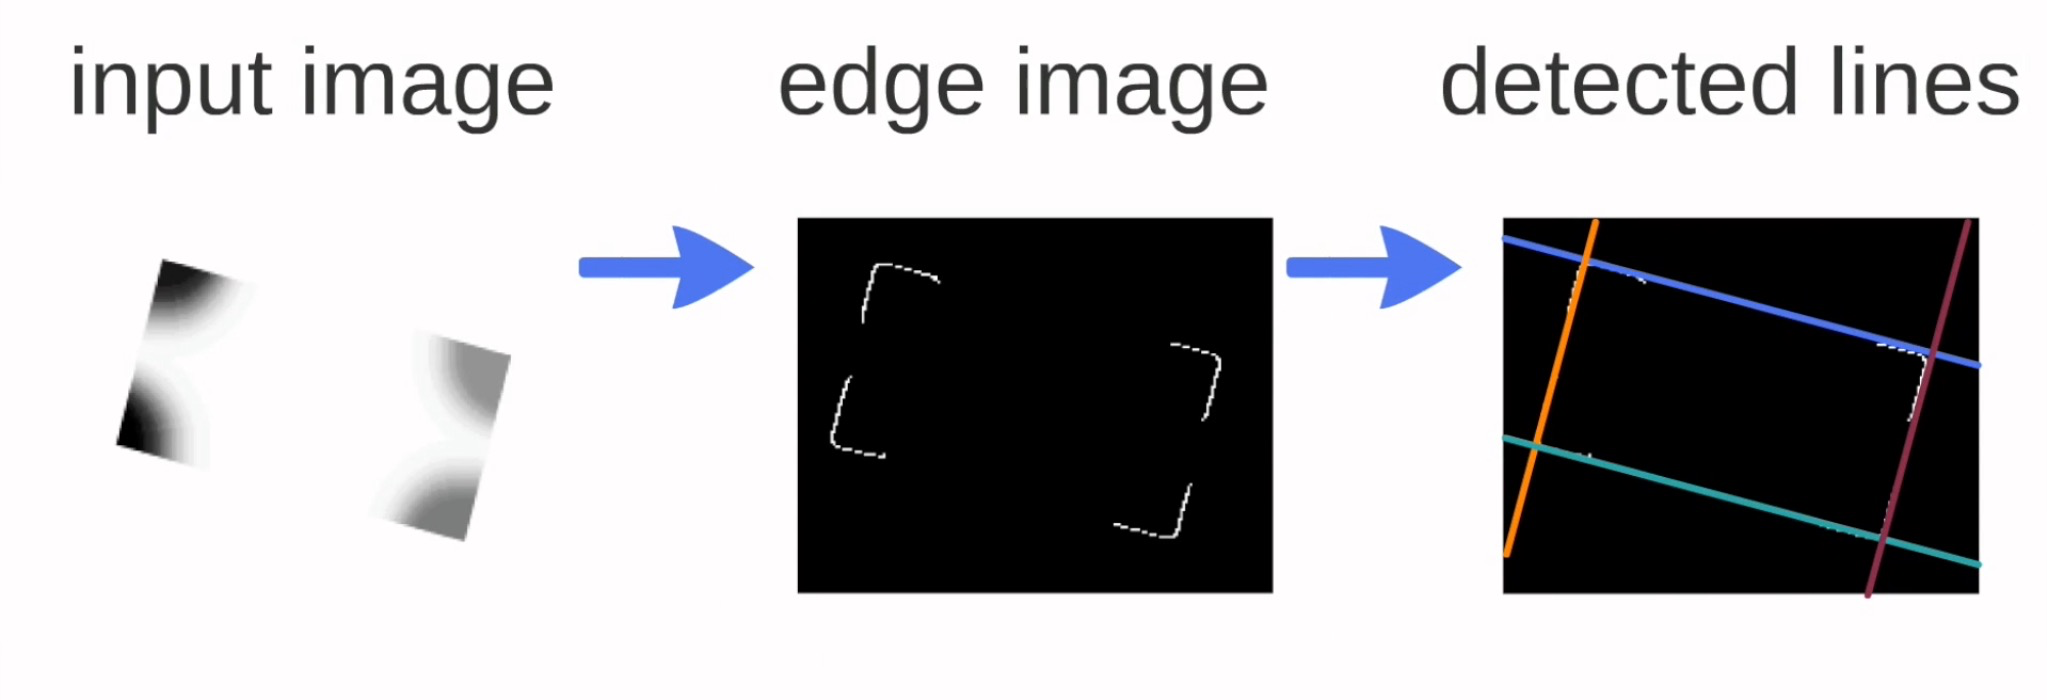
\includegraphics[height=4cm]{images/hough_1.png}
\end{center}

\subsubsection{Premi\`ere approche}

\paragraph{Repr\'esentation d'une droite}
La formule la plus simple repr\'esentant une droite dans le plan est son \'equation cart\'esienne et r\'eduite $y=ax+b$ (avec $a, b \in \mathbb{R}$) où
$$\begin{cases}
a$ est la pente de la droite$ \\
b$ est l'ordonn\'ee \`a l'origine$
\end{cases}$$

\begin{center}
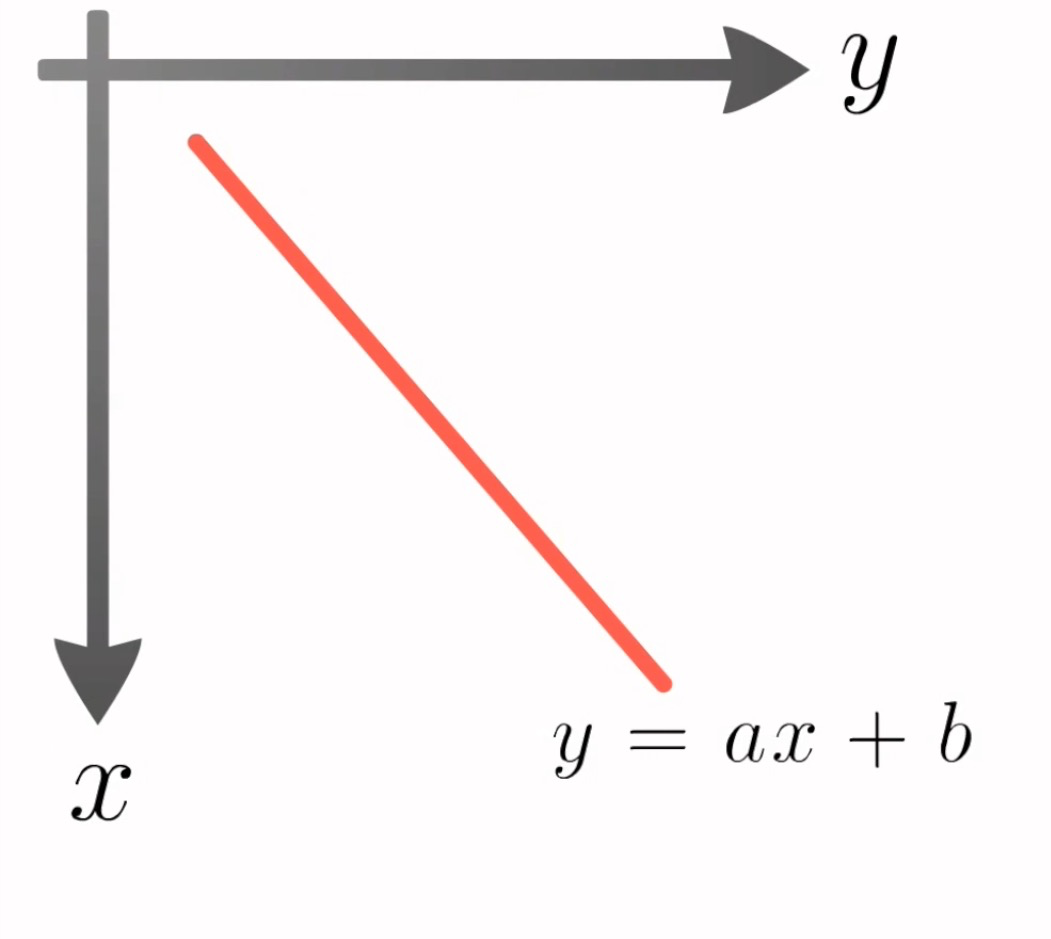
\includegraphics[height=3cm]{images/hough_2.png}
\end{center}
Toutes les droites passant par un point de coordonn\'ees $(x_1, y_1)$ fix\'ees ont la forme $y_1=ax_1+b$ pour diff\'erentes valeurs de $a$ et $b$. 
\begin{center}
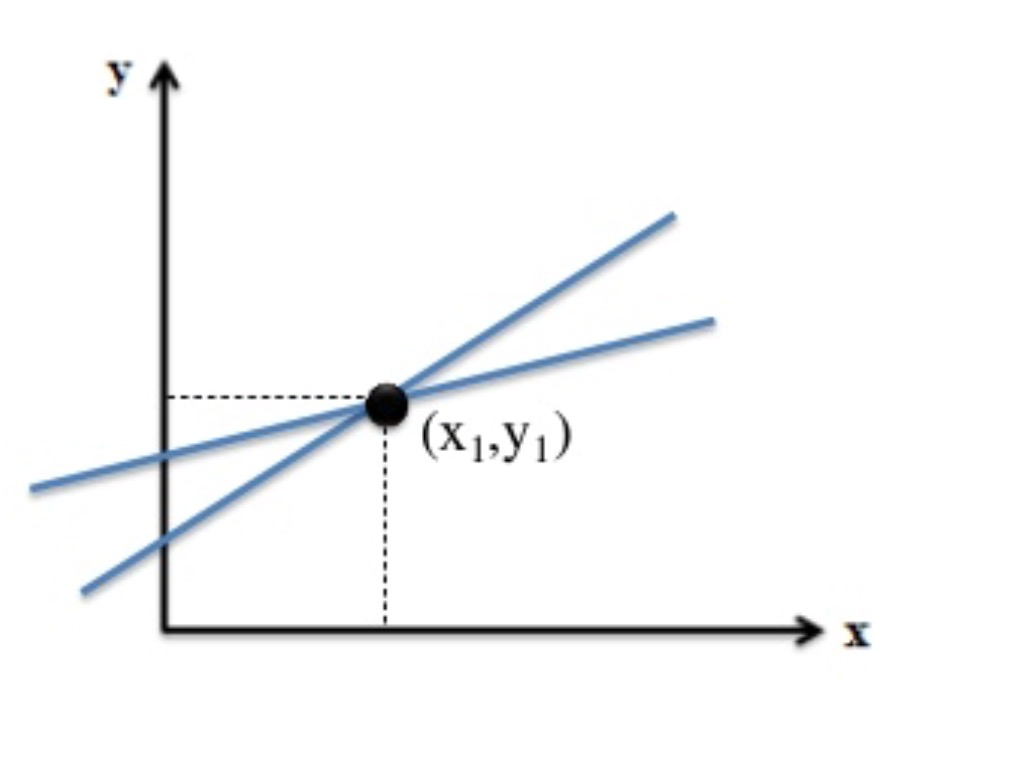
\includegraphics[height=3cm]{images/hough_8.png}
\end{center}

\paragraph{Principe d\'etaill\'e}
On va changer le rep\`ere en rempla\c cant $x$ par $a$ et $y$ par $b$.
Chaque droite dans l'espace $(x, y)$ sera transform\'ee en un point dans l'espace $(a, b)$, espace de Hough.
Invers\'ement, chaque point dans l'espace $(x, y)$ sera transform\'e en une droite d'\'equation $b=-ax+y$ dans l'espace de Hough.
\begin{center}
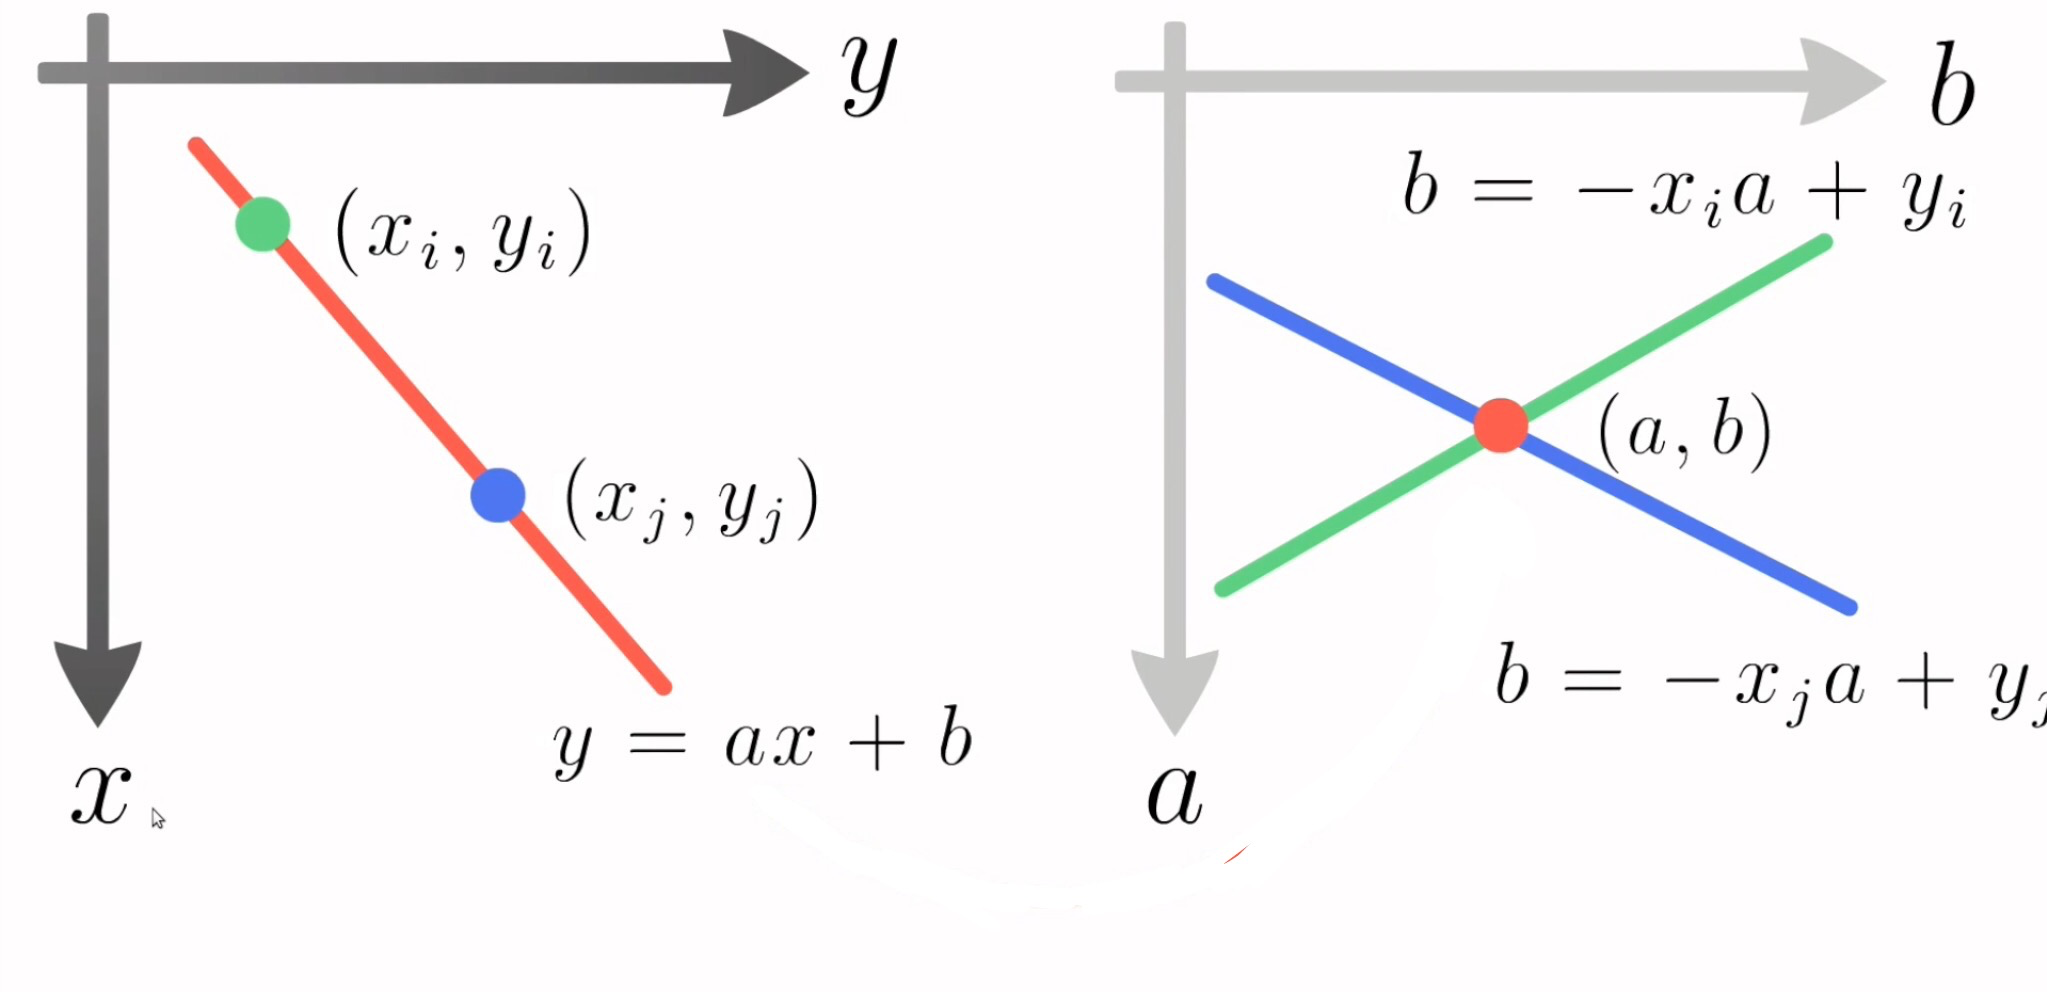
\includegraphics[height=3cm]{images/hough_3.png}
\end{center}
Pour un point $A$, toutes les droites passant par ce point correspondent \`a une seule droite $a$ dans l'espace de Hough. \\
Pour un point $B$, toutes les droites passant par ce point correspondent \`a une seule droite $b$ dans l'espace de Hough. \\
Ces $2$ faisceaux de droites dans l'espace $(x, y)$ ont en commun l'unique droite qui relie $A$ et $B$. \\
Cette droite correspond, dans l'espace de Hough, au point qui est l'intersubsection des $2$ droites $a$ et $b$. \\
Cette intersection, ce point contient les param\`etres de la droite recherch\'ee. \\
 \\
Tous les points situ\'es sur une m\^eme droite $c$ dans l'espace $(x, y)$ sont repr\'esent\'es par des droites passant toutes par un m\^eme point $C$ dans l'espace de Hough. \\
Les coordonn\'ees de ce point $C(x_c, y_c)$ contiennent les param\`etres recherch\'es de la droite $c \equiv y=x_cx+y_c$ \\
 \\
Il existe un principe de vote : on utilise un accumulateur o\`u chaque point peut voter pour une droite particuli\`ere et les droites recevant le plus de votes sont conserv\'ees. \\
On ne va cependant pas d\'evelopper ce principe ici. \\
 \\
Cette repr\'esentation $y=ax+b$ pose un probl\`eme pour les droites verticales.  Voil\`a pourquoi la repr\'esentation suivante, qui r\`egle ce probl\`eme, est la plus utilis\'ee.

\subsubsection{Approche trigonom\'etrique}

\paragraph{Repr\'esentation polaire d'une droite}
Une droite peut aussi \^etre repr\'esent\'ee par la formule $y\sin\theta+x\cos\theta=\rho$ (avec $\theta \in [-\pi/2 ; \pi/2]$ et $\rho \in [0 ; d]$ où $d$ est la longueur de la diagonale de l'image)  o\`u

$$\begin{cases}
\theta$ est l'angle entre l'axe $x$ et le vecteur $\vec\rho \\
\rho$ est la distance la plus courte entre l'origine du rep\`ere et la droite$
\end{cases}$$

\begin{center}
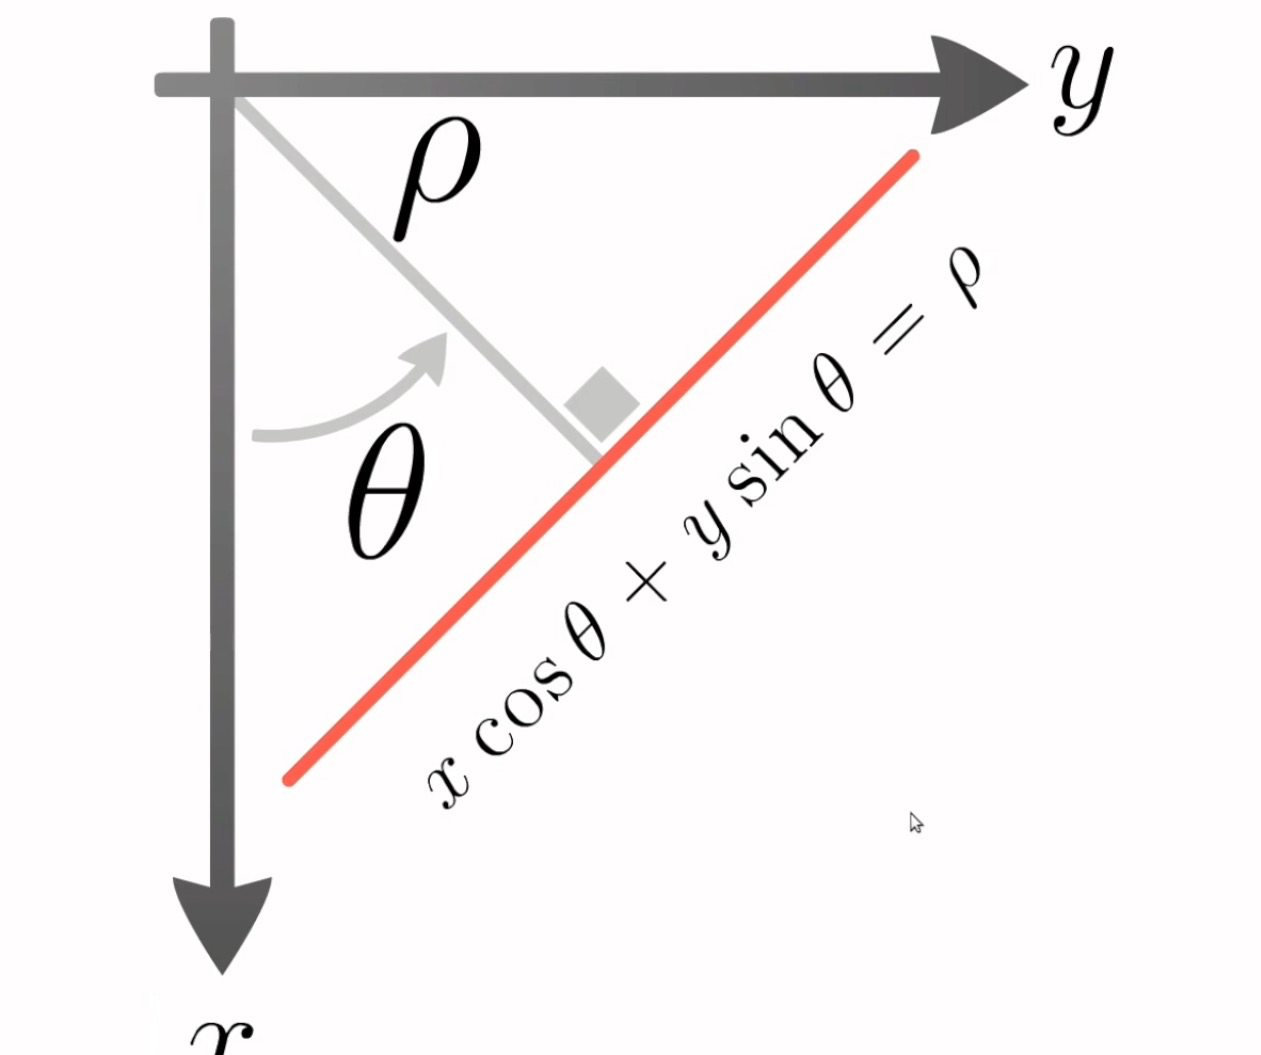
\includegraphics[height=3cm]{images/hough_4.png}
\end{center}

\paragraph{Principe d\'etaill\'e}
On change \'egalement le rep\`ere en rempla\c cant $x$ par $\theta$ et $y$ par $\rho$ : \\
Chaque droite dans l'espace $(x, y)$ sera transform\'ee en un point dans l'espace $(\rho, \theta)$. \\
Chaque point dans l'espace $(x, y)$ sera transform\'e en une courbe, une sinuso\"ide dans l'espace $(\rho, \theta)$. \\
 \\
Les points d'intersubsection des sinuso\"ides dans l'espace $(\rho, \theta)$ sont utilis\'es pour trouver les droites dans l'espace $(x, y)$. \\
 \\
La transform\'ee de Hough fait ensuite appel \`a un algorithme qui regarde tous les points et imagine toutes les valeurs possibles pour $\rho$ et $\theta$. \\
On observe, dans l'espace $(\rho, \theta)$, des pics pour les valeurs qui reviennent le plus souvent et l'algorithme va d\'efinir les droites dans l'espace $(x, y)$ et donc les lignes d\'etect\'ees dans l'image.
\begin{center}
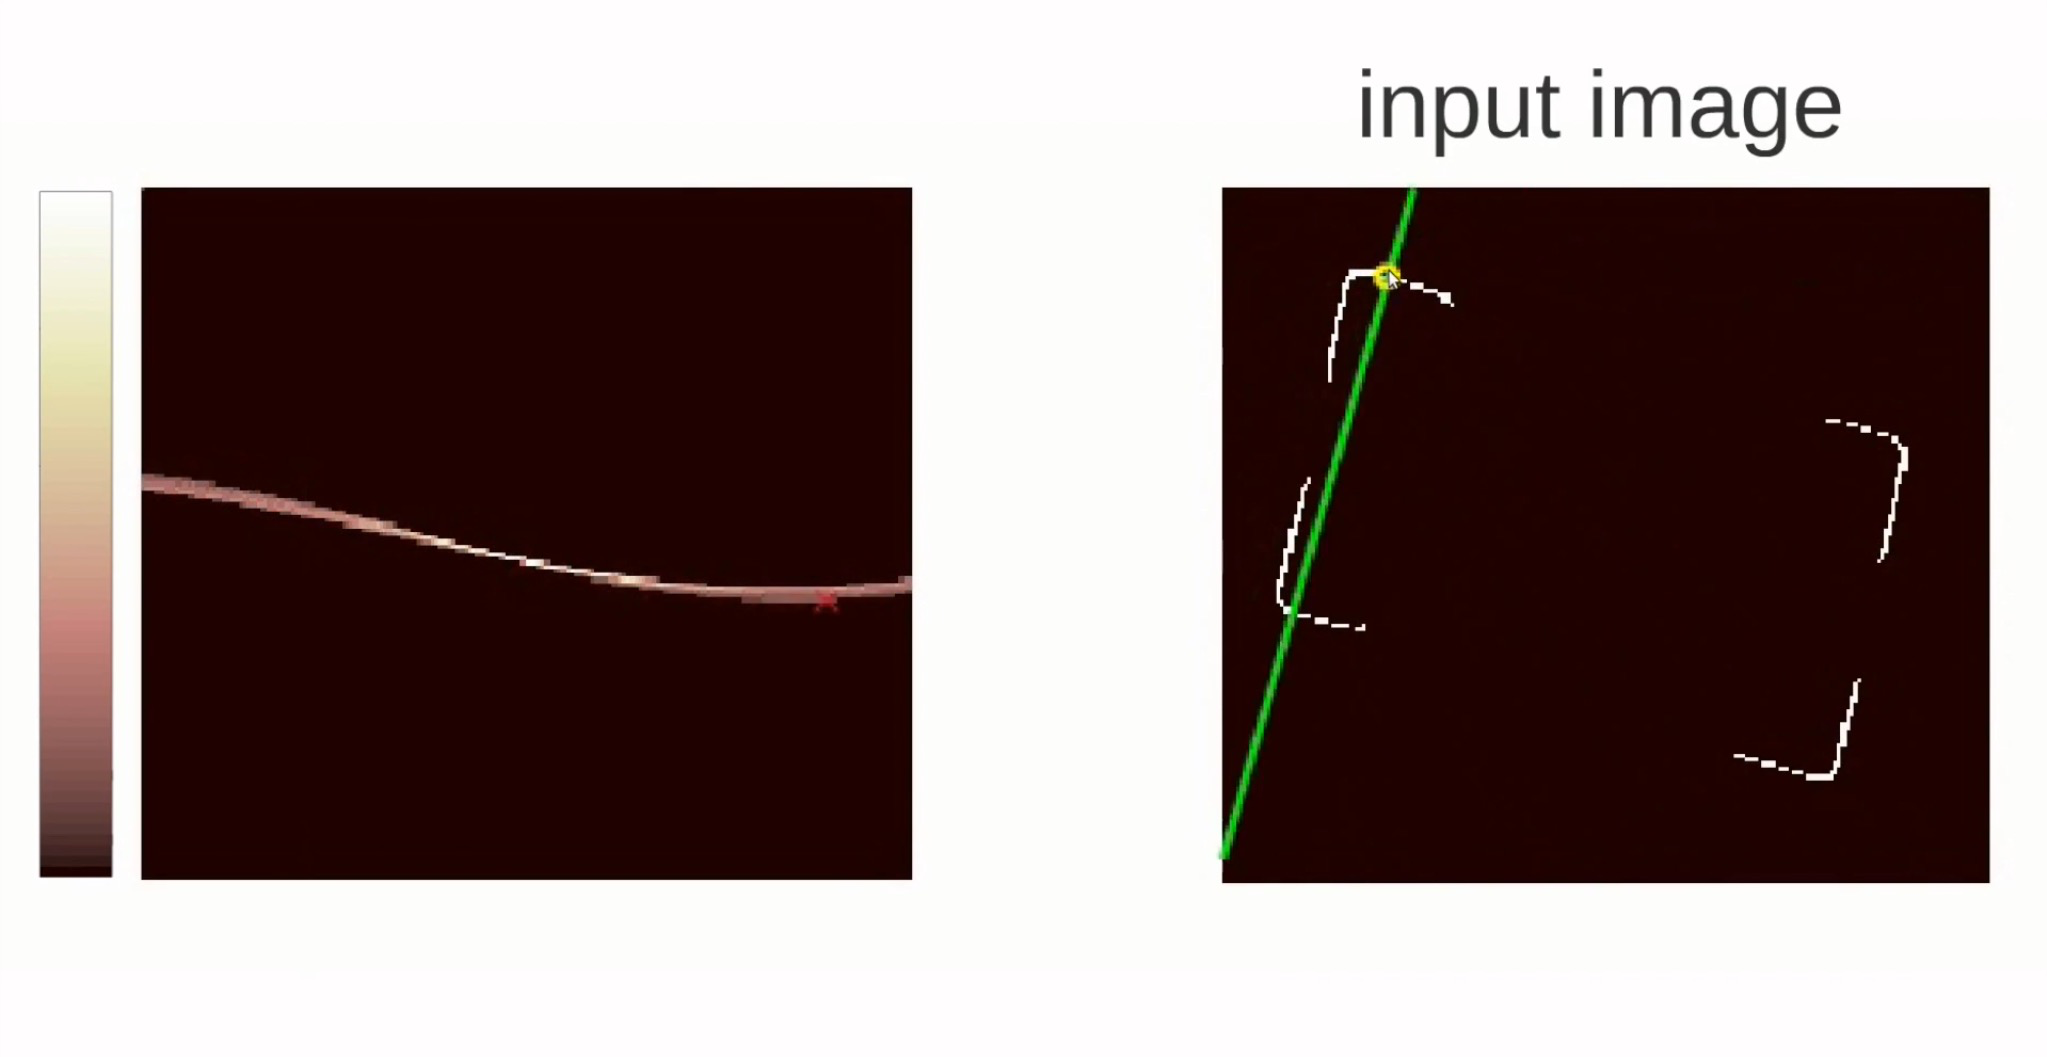
\includegraphics[height=3cm]{images/hough_5.png} \\
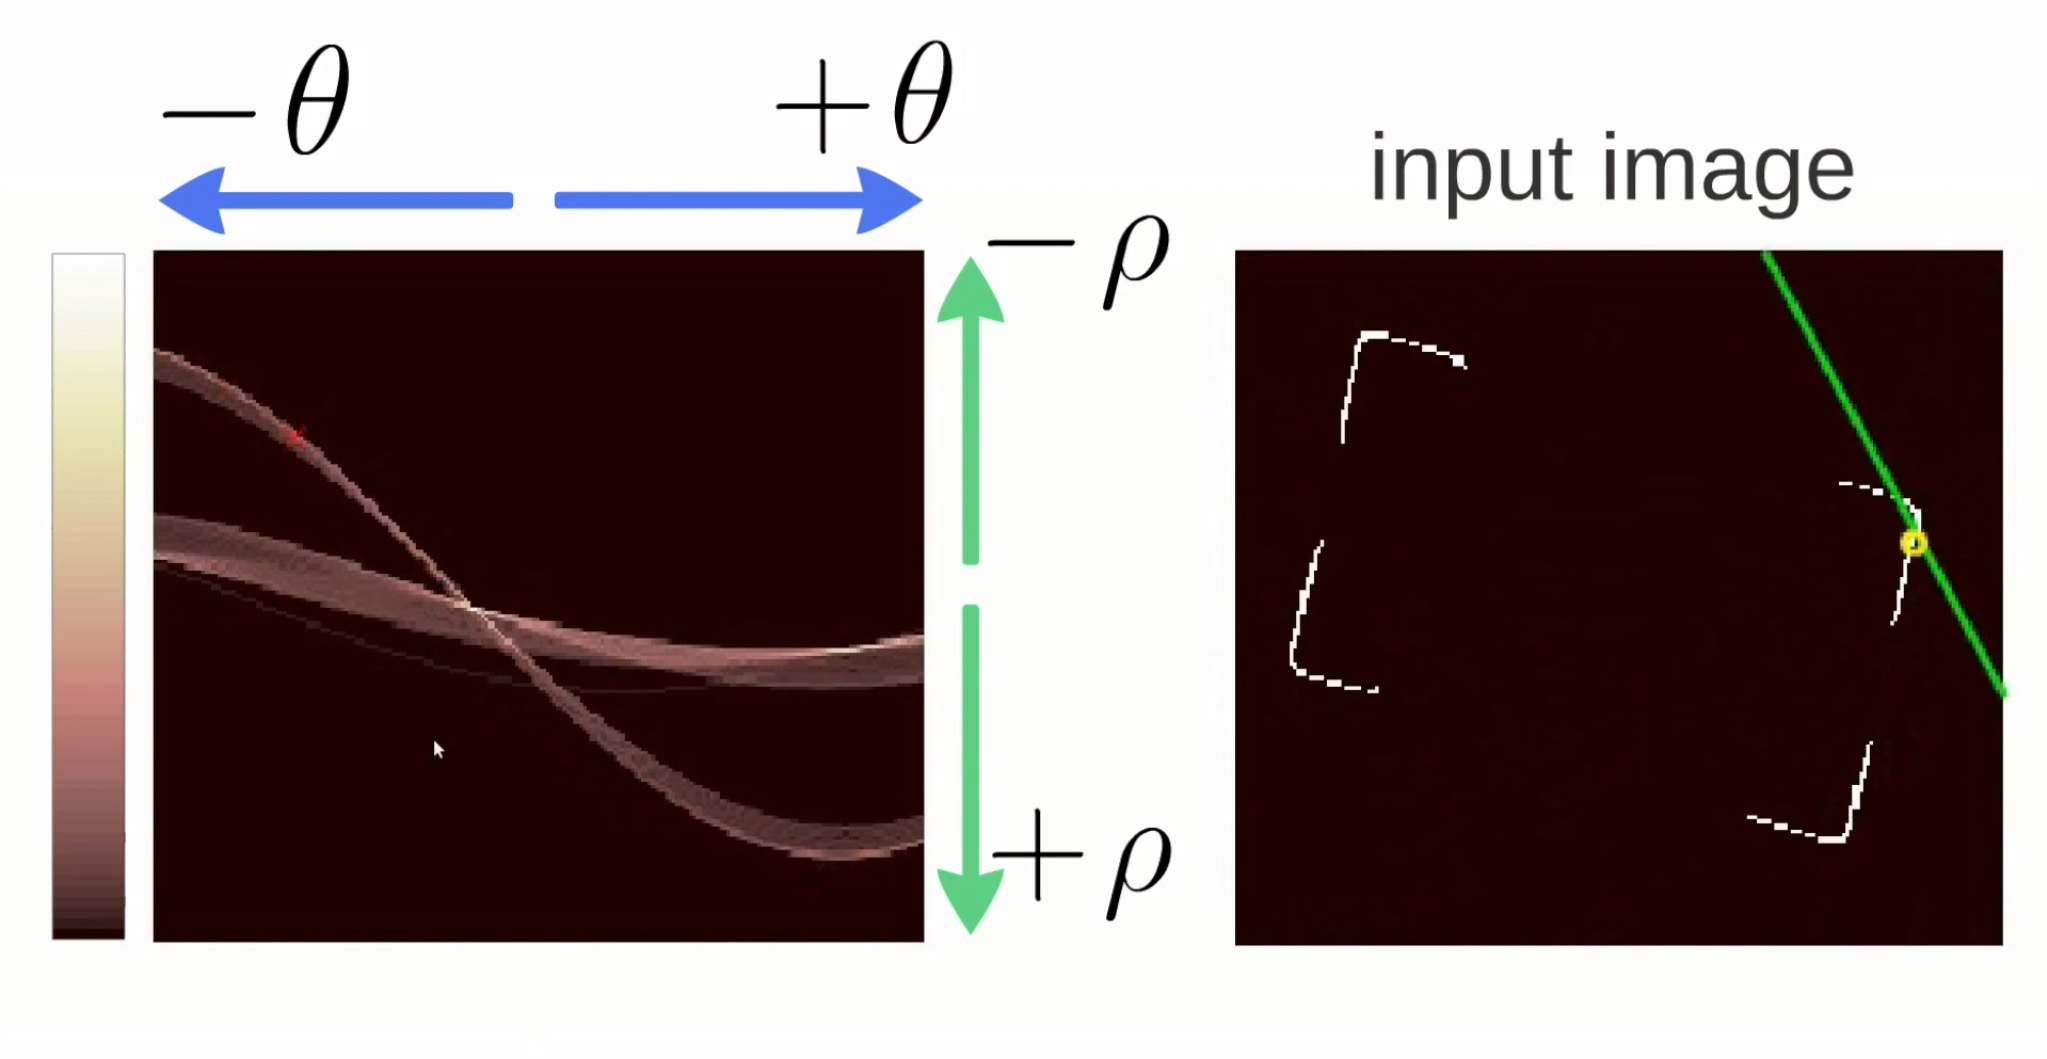
\includegraphics[height=3cm]{images/hough_6.png} \\ 
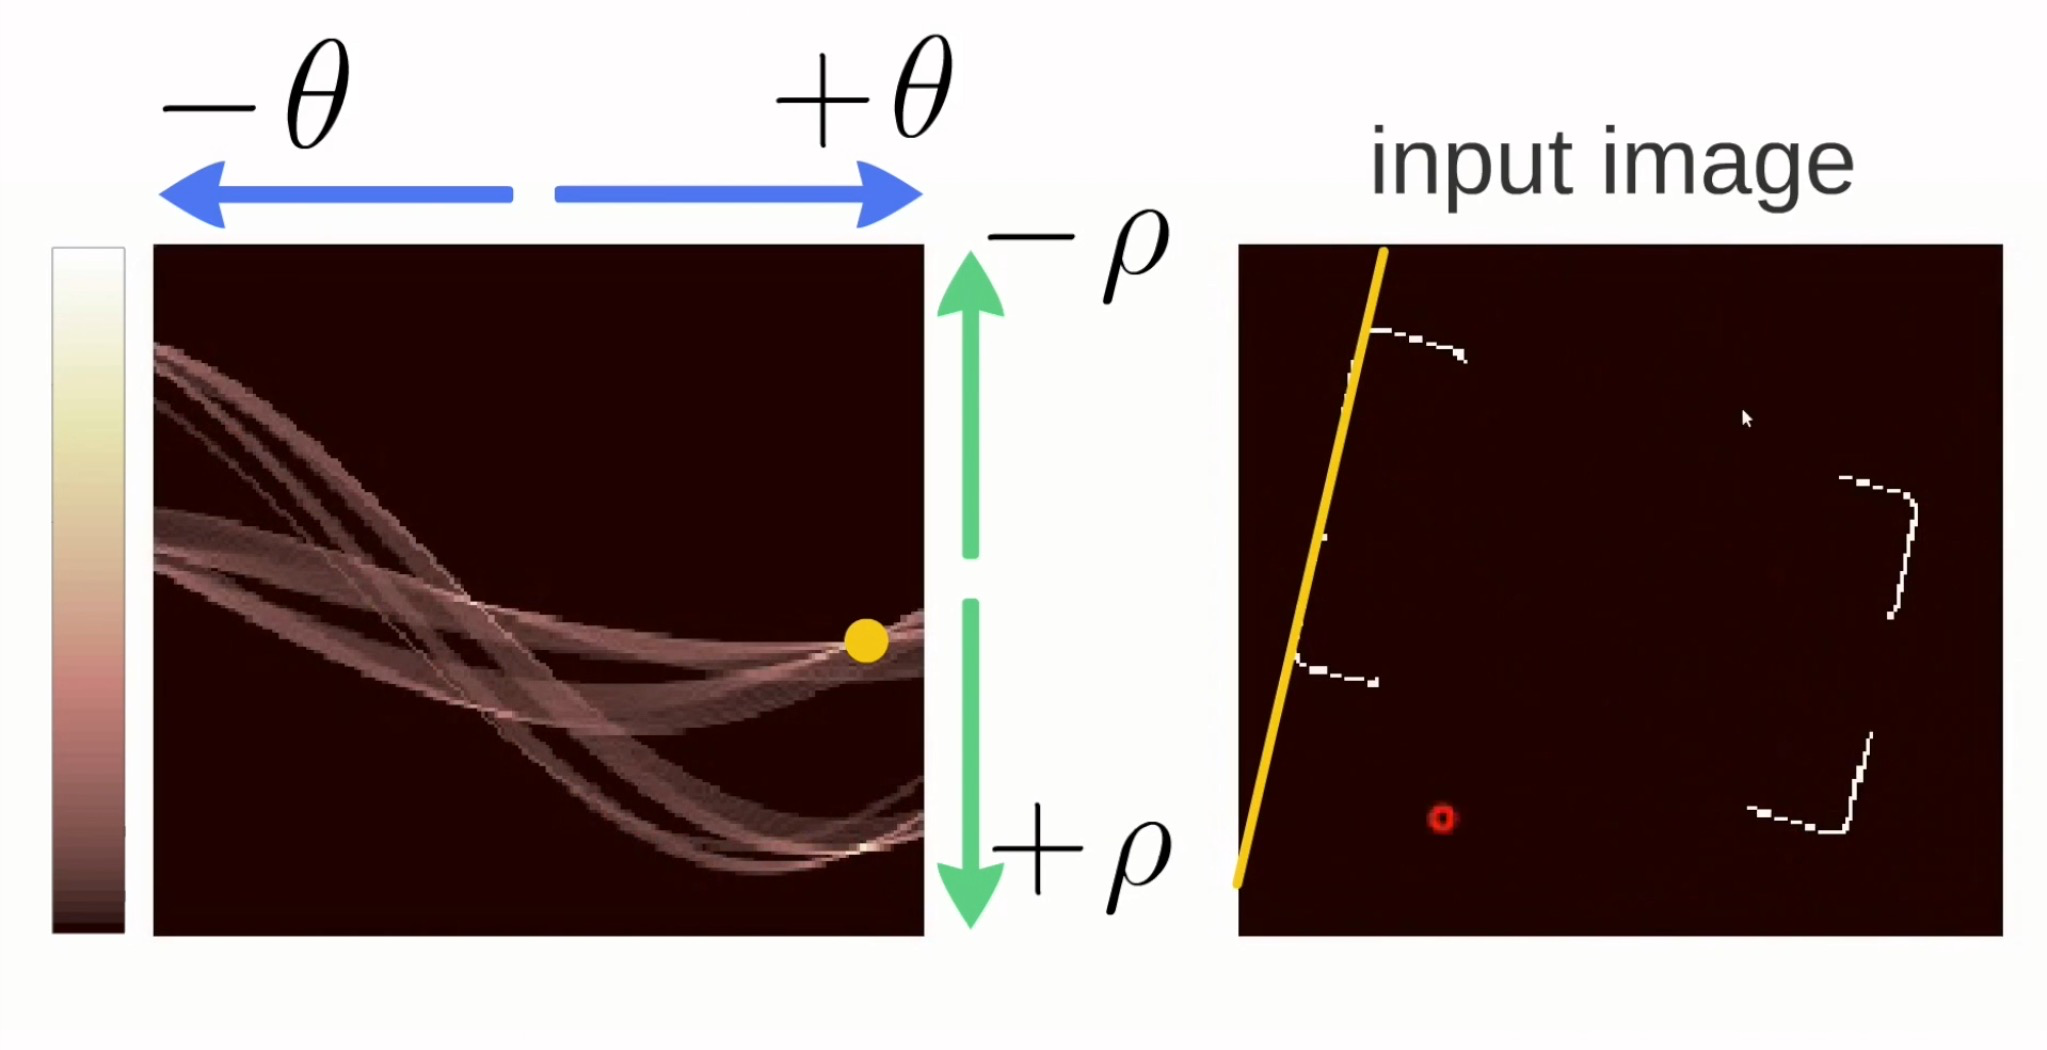
\includegraphics[height=3cm]{images/hough_7.png}
\end{center}

\subsubsection{Conclusion}
La transform\'ee de Hough est un outil efficace pour trouver les lignes dans une image. \\
Il existe d'autres transform\'ees de Hough pour extraire d'autres formes. \\
Elle est utilis\'ee dans plusieurs applications : d\'etection de routes dans les images prises par satellite, lecture de codes barres...